\chapter{Análise Estatística Não Paramétrica}
\label{chap:analise_estatistica_np}
Considerando que as distribuições das métricas de conectividade (diferença entre Pós e Pré) não se comportam de maneira normal (ver Capítulo~\ref{chap:analise_distribuicao_normalidade}), optamos por empregar testes estatísticos não paramétricos para comparar as condições de estimulação \textit{cathodic} \textit{versus} \textit{sham}. Essa escolha evita pressupostos inadequados sobre a distribuição dos dados. Além da violação de normalidade, a presença de \textit{outliers} reforça a adoção de testes não paramétricos neste cenário de heterogeneidade amostral.

Nesta etapa, foram aplicados os seguintes testes:
\begin{itemize}
    \item \textbf{Mann-Whitney U}: teste para amostras independentes, usado para avaliar se as distribuições das diferenças entre ``\textit{cathodic}'' e ``\textit{sham}'' diferem significativamente em cada faixa de frequência e grupo de canais.  
      O tamanho de efeito foi calculado como correlação bisserial de postos:
      \[
        r_{rb} = \frac{2U}{n_1\,n_2} - 1,
      \]
      onde \(U\) é a estatística de Mann-Whitney e \(n_1,n_2\) são os tamanhos das amostras. Varia de \(-1\) a \(+1\):  
      \(\,r_{rb}>0\) indica que ``cathodic'' tende a valores maiores que ``sham'' e \(r_{rb}<0\) o inverso.
      
    \item \textbf{Kruskal-Wallis}: teste para amostras independentes, matematicamente equivalente ao Mann-Whitney U quando há apenas duas amostras.  
      O tamanho de efeito foi calculado como
      \[
        \eta = \frac{H}{n_1 + n_2 - 1},
      \]
      onde \(H\) é a estatística de Kruskal-Wallis. Varia de 0 a 1, representando apenas a magnitude do efeito (sem sinal direcional).
      
    \item \textbf{Wilcoxon signed-rank}: teste para amostras pareadas, que compara Pré \textit{versus} Pós em cada atleta e par de canais, capturando mudanças intraindividuais. O tamanho de efeito foi calculado como
      \[
        r = \frac{W}{n(n+1)/2},
      \]
      onde \(W\) é a soma de postos e \(n\) o número de pares. Varia de 0 a 1 e indica apenas magnitude (sem sinal); para direção consulte a análise bootstrap na Seção \ref{sec:effect_size_distribution}.
  \end{itemize}

Os testes foram realizados separadamente para cada métrica de conectividade (\textit{median\_plv\_diff}, \textit{median\_pli\_diff} e \texttt{median\_cf\_plm\_diff}) e para os grupos de canais \texttt{EEG\_EEG} e \texttt{EEG\_ECG}. Embora o código inclua remoção de dados nulos, na prática não houve valores faltantes.

Em todo o conjunto de comparações (5 bandas × 2 grupos de canais = 10 testes), aplicamos Bonferroni
\[ 
  \alpha_{\mathrm{corr}} \;=\; \frac{0{,}05}{10} \;=\; 0{,}005 \,,
\]
ou seja, consideramos significativos apenas os testes com \(p_{\rm raw}<0{,}005\).

\section{Detecção de \textit{Outliers}, Análise \textit{Bootstrap} e Correções para Comparações Múltiplas}
Para avaliar o impacto dos pontos atípicos nas análises subsequentes, optamos por realizar uma etapa adicional de detecção e remoção de \textit{outliers} utilizando o método ECOD, especialmente adequado ao nosso conjunto de dados devido à sua natureza não paramétrica, identificando anomalias sem pressupor uma distribuição específica dos dados. Estudos demonstram que o ECOD supera diversas técnicas convencionais de detecção de \textit{outliers} em termos de acurácia e eficiência \cite{li2022ecod}.

Aplicamos o ECOD considerando as métricas \textit{median\_pli\_diff} e \texttt{median\_cf\_plm\_diff}. Inicialmente, o dataset continha 122915 entradas; após a aplicação do ECOD, aproximadamente 5,00\% dos dados foram identificados como \textit{outliers} e removidos. Paralelamente, todo o mesmo conjunto de análises foi executado sem remover os outliers, e esses resultados ``sem remoção'' são apresentados nas seções subsequentes.

Posteriormente, implementamos um pipeline de análise baseado em \textit{Bootstrap} acelerado por placa de vídeo (GPU) para o cálculo de intervalos de confiança \textit{Bias-Corrected and Accelerated} (BCa). Esse método é particularmente robusto, pois ajusta tanto o viés quanto a aceleração da distribuição \textit{bootstraped}, permitindo capturar assimetrias e a influência residual de \textit{outliers} nos dados. Embora computacionalmente custoso, o método BCa é amplamente reconhecido como uma das abordagens mais precisas para a estimação de intervalos de confiança em situações onde os pressupostos de normalidade não são atendidos. Optamos por esse método em detrimento de outras técnicas devido à sua capacidade de corrigir distorções na distribuição da estatística estimada.

Para avaliar a significância estatística após múltiplas comparações, utilizamos a função \textit{multipletests} da biblioteca Python \textit{statsmodels} com o método Bonferroni. Este procedimento ajusta os p-valores originais multiplicando-os pelo número total de comparações realizadas, tornando o critério de significância mais conservador e minimizando o risco de falsos positivos. Dessa forma, efeitos são considerados significativos quando o p-valor corrigido por Bonferroni for inferior a 0,05.

Além disso, nosso pipeline incluiu o cálculo de tamanhos de efeito utilizando diversas métricas, tais como:
\begin{itemize}
    \item Cohen's \(d\) e Hedges' \(g\): que quantificam a magnitude da diferença entre as condições em termos de desvios-padrão;
    \item \textit{Rank-Biserial Correlation} (RBC): derivado do teste de Wilcoxon, que fornece uma interpretação robusta baseada em postos.
\end{itemize}

Essas métricas complementares permitem uma avaliação abrangente do efeito da estimulação e possibilitam comparar os resultados obtidos com diferentes abordagens, como o método de Bonferroni, Holm e \textit{False Discovery Rate-Benjamini-Hochberg} (FDR-BH), fornecendo uma visão diversificada dos achados.

Em resumo, nossa abordagem compreende as seguintes etapas:
\begin{enumerate}
    \item \textbf{Detecção de \textit{Outliers} e análise paralela sem remoção}: Usamos o ECOD para identificar e remover \(d\approx5\)\%  dos dados anômalos, mas também mantivemos um pipeline paralelo sem remoção de outliers; ambos os conjuntos de resultados são explorados nas seções seguintes.
    \item \textbf{Análise \textit{Bootstrap} com GPU:} Implementamos o cálculo de intervalos de confiança BCa, estimando viés, erro padrão e tamanhos de efeito por meio de reamostragem acelerada, assegurando precisão mesmo em distribuições assimétricas.
    \item \textbf{Testes Não Paramétricos e Correção para Comparações Múltiplas:} Aplicamos testes não paramétricos, como o teste de Wilcoxon para dados emparelhados, e corrigimos os p-valores utilizando o método Bonferroni (além de outras correções complementares), minimizando o risco de erros do tipo I.
\end{enumerate}

Devido ao grande número de comparações realizadas, apresentamos aqui um sumário estatístico dos resultados significativos. As tabelas completas com todos os resultados individuais estão disponíveis publicamente em nosso repositório GitHub \cite{barros2025repository} (\url{https://github.com/dantebarross/efeito-da-neuromodulacao-na-sincronicidade-eeg-ecg}). As Tabelas \ref{tab:summary_eeg_eeg_with} e \ref{tab:summary_eeg_eeg_without} apresentam os resultados sumarizados para as comparações EEG-EEG, com e sem outliers, respectivamente. e as Tabelas \ref{tab:summary_eeg_ecg_with} e \ref{tab:summary_eeg_ecg_without} mostram os resultados para as comparações EEG-ECG.

As tabelas de resumo fornecem apenas uma visão geral dos resultados, sem aprofundar nos resultados individuais observados. Na próxima seção, exploramos esses achados em detalhes por meio de gráficos que ilustram as distribuições dos tamanhos de efeito (Cohen's \(d\), Hedges' \(g\) e correlação de postos Wilcoxon RBC) e dos p-valores. Em seguida, no Capítulo~\ref{chap:analise_de_rede}, apresentamos mapas de conectividade (visualizações em redes topográficas) para todos os grupo de canais e faixas de frequência.

\inputtable{tabelas/summary_eeg_eeg_with_outliers.tex}
{Sumário estatístico das comparações EEG-EEG com outliers}
{summary_eeg_eeg_with}
{Elaborado pelo autor (2025)}

\inputtable{tabelas/summary_eeg_eeg_without_outliers.tex}
{Sumário estatístico das comparações EEG-EEG sem outliers}
{summary_eeg_eeg_without}
{Elaborado pelo autor (2025)}

\inputtable{tabelas/summary_eeg_ecg_with_outliers.tex}
{Sumário estatístico das comparações EEG-ECG com outliers}
{summary_eeg_ecg_with}
{Elaborado pelo autor (2025)}

\inputtable{tabelas/summary_eeg_ecg_without_outliers.tex}
{Sumário estatístico das comparações EEG-ECG sem outliers}
{summary_eeg_ecg_without}
{Elaborado pelo autor (2025)}

\section{Distribuição de Tamanhos de Efeito e p-valores}
\label{sec:effect_size_distribution}
Nesta etapa, examinamos a distribuição das estimativas de tamanho de efeito (Cohen's \(d\), Hedges' \(g\)  e Wilcoxon RBC) e dos p-valores (brutos e corrigidos por Bonferroni) para as análises de PLI (EEG-EEG) e CF-PLM (EEG-ECG), considerando cenários com e sem \textit{outliers}. 

A Figura~\ref{fig:effectsizehist_all} ilustra, em quatro subfiguras, como essas métricas se distribuem ao longo dos pares de canal e faixas de frequência analisados.

\begin{figure}[htb]
    \centering
    % Subfigura 1: PLI (EEG-EEG), Sem Outliers
    \subfloat[Sem Outliers - PLI (EEG-EEG)]{
        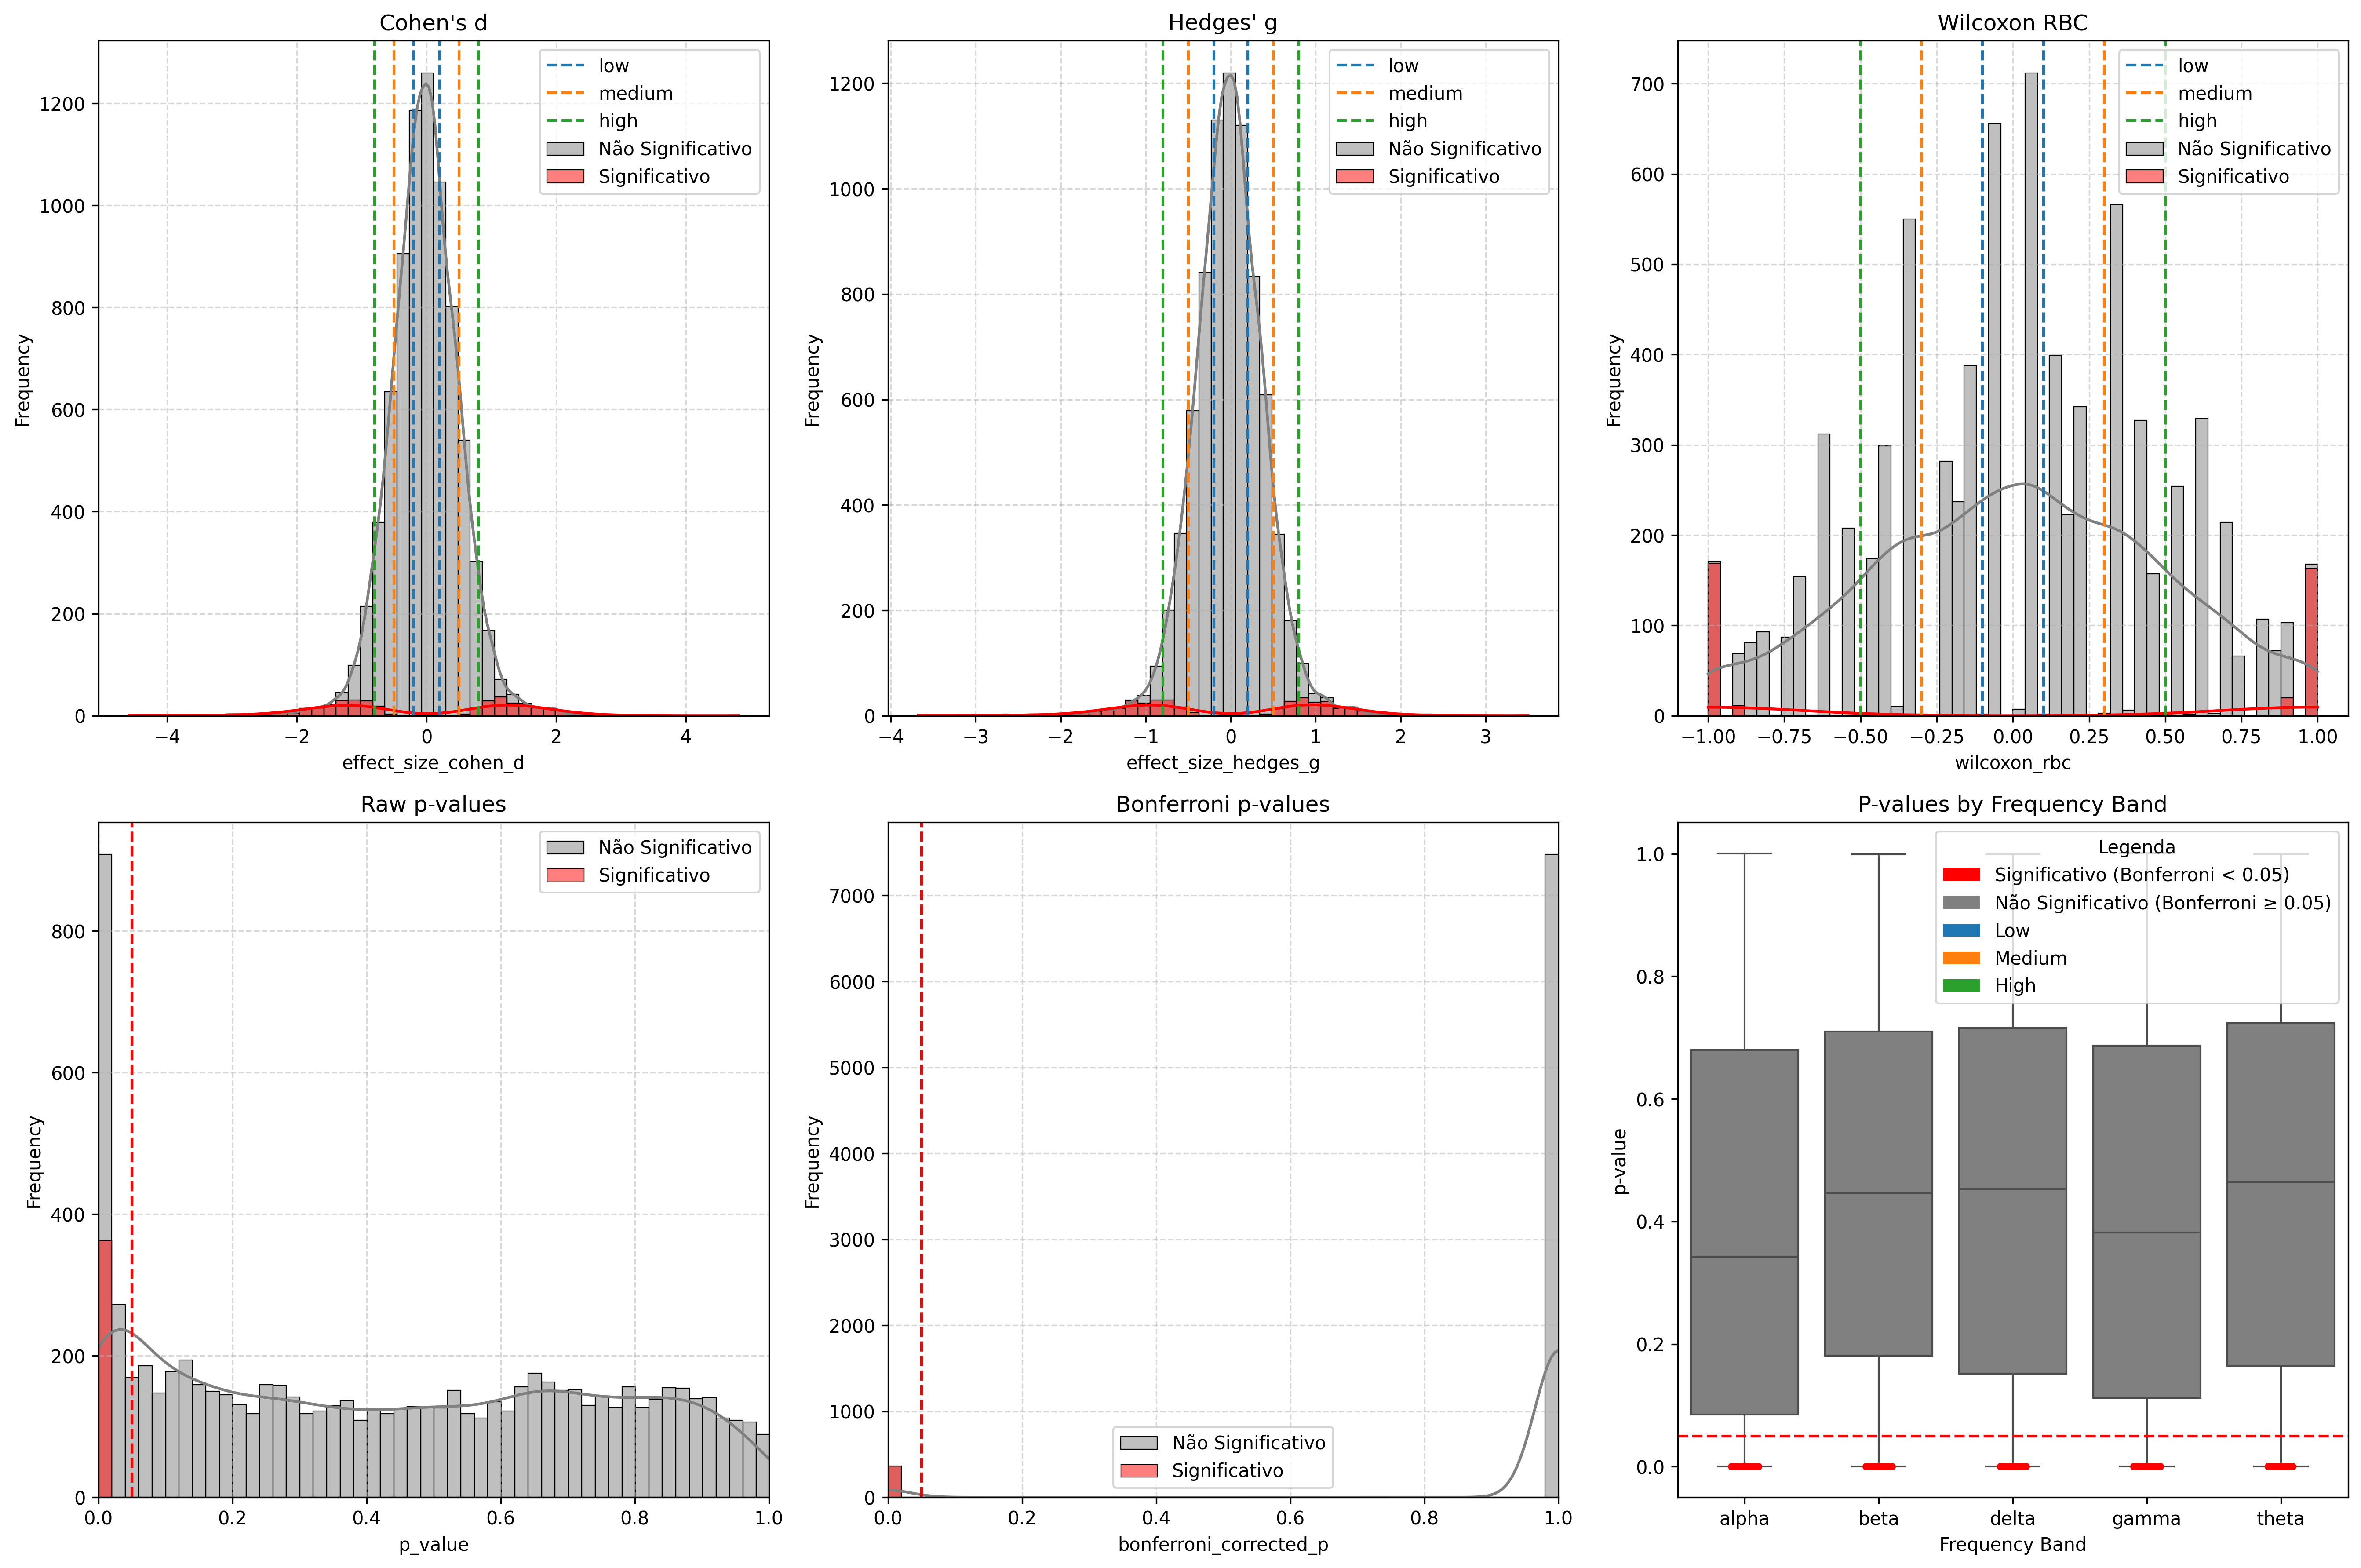
\includegraphics[width=0.45\textwidth]{figs/7_bootstrap_results_analysis/1_effect_size_histograms/Effect_Size_Histograms_PLI_EEGEEG_Sem_Outliers.png}
    }
    \quad
    % Subfigura 2: CF-PLM (EEG-ECG), Sem Outliers
    \subfloat[Sem Outliers - CF-PLM (EEG-ECG)]{
        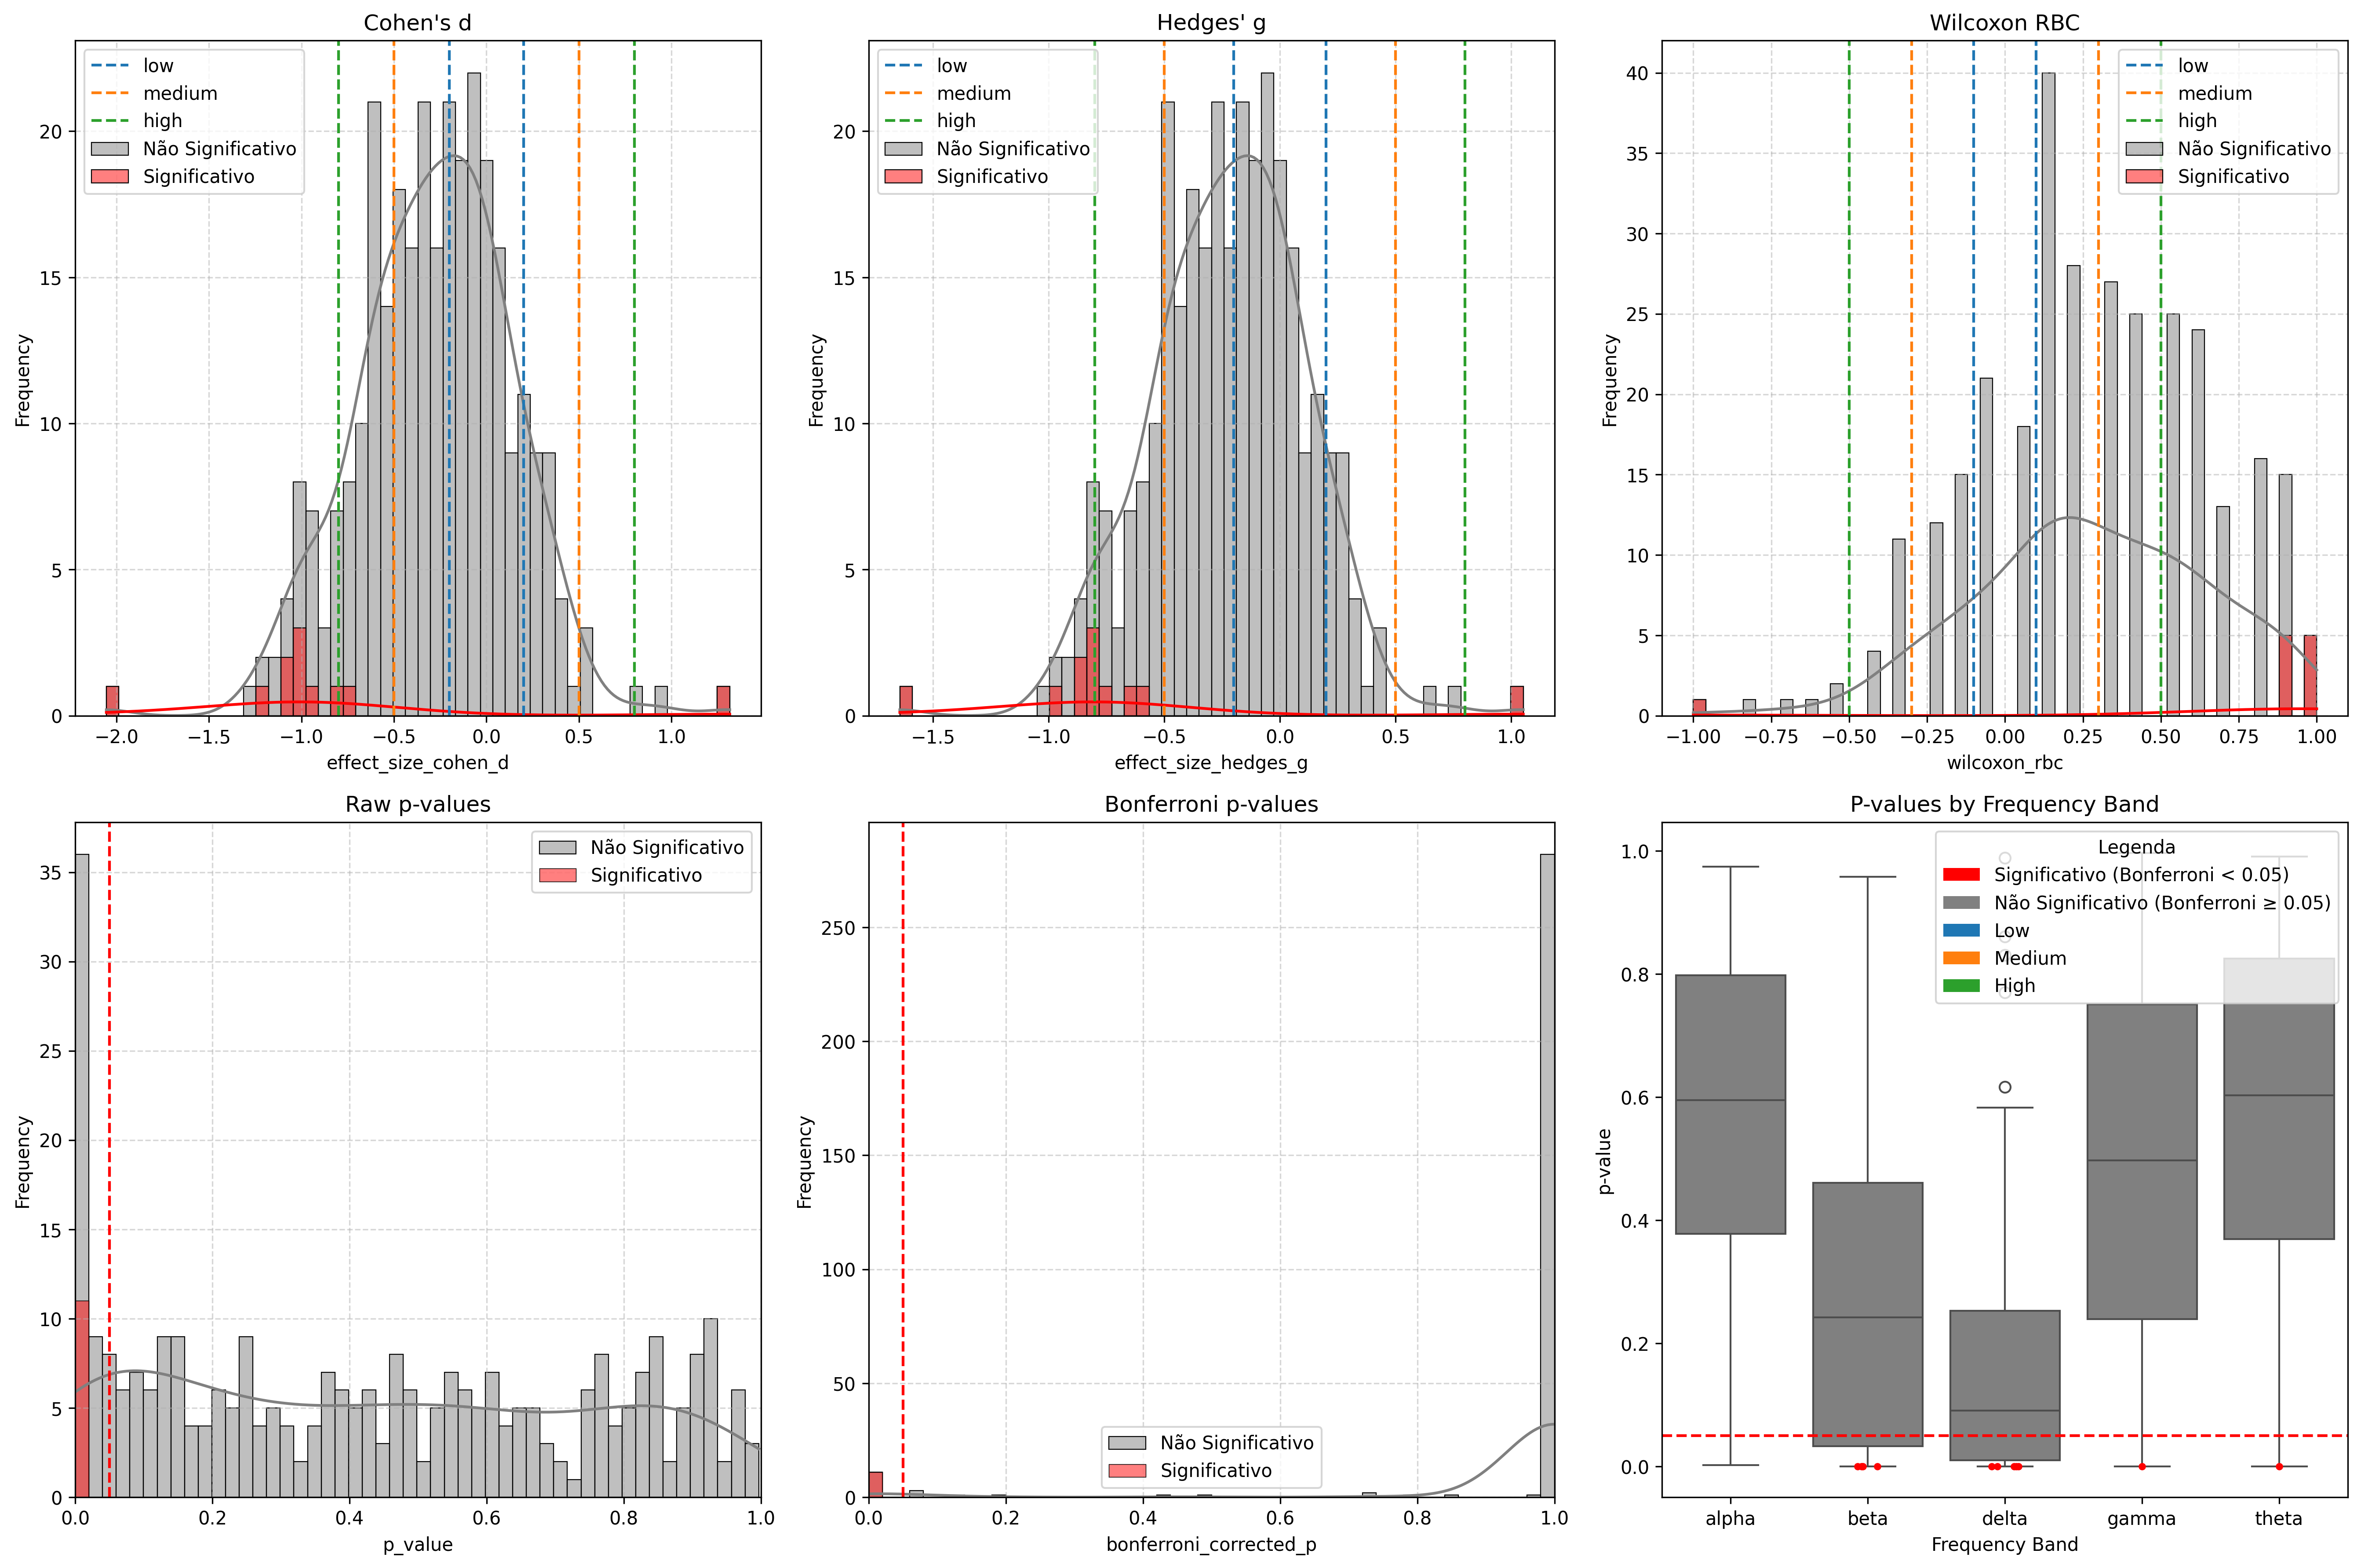
\includegraphics[width=0.45\textwidth]{figs/7_bootstrap_results_analysis/1_effect_size_histograms/Effect_Size_Histograms_CFPLM_EEGECG_Sem_Outliers.png}
    }
    \\
    % Subfigura 3: PLI (EEG-EEG), Com Outliers
    \subfloat[Com Outliers - PLI (EEG-EEG)]{
        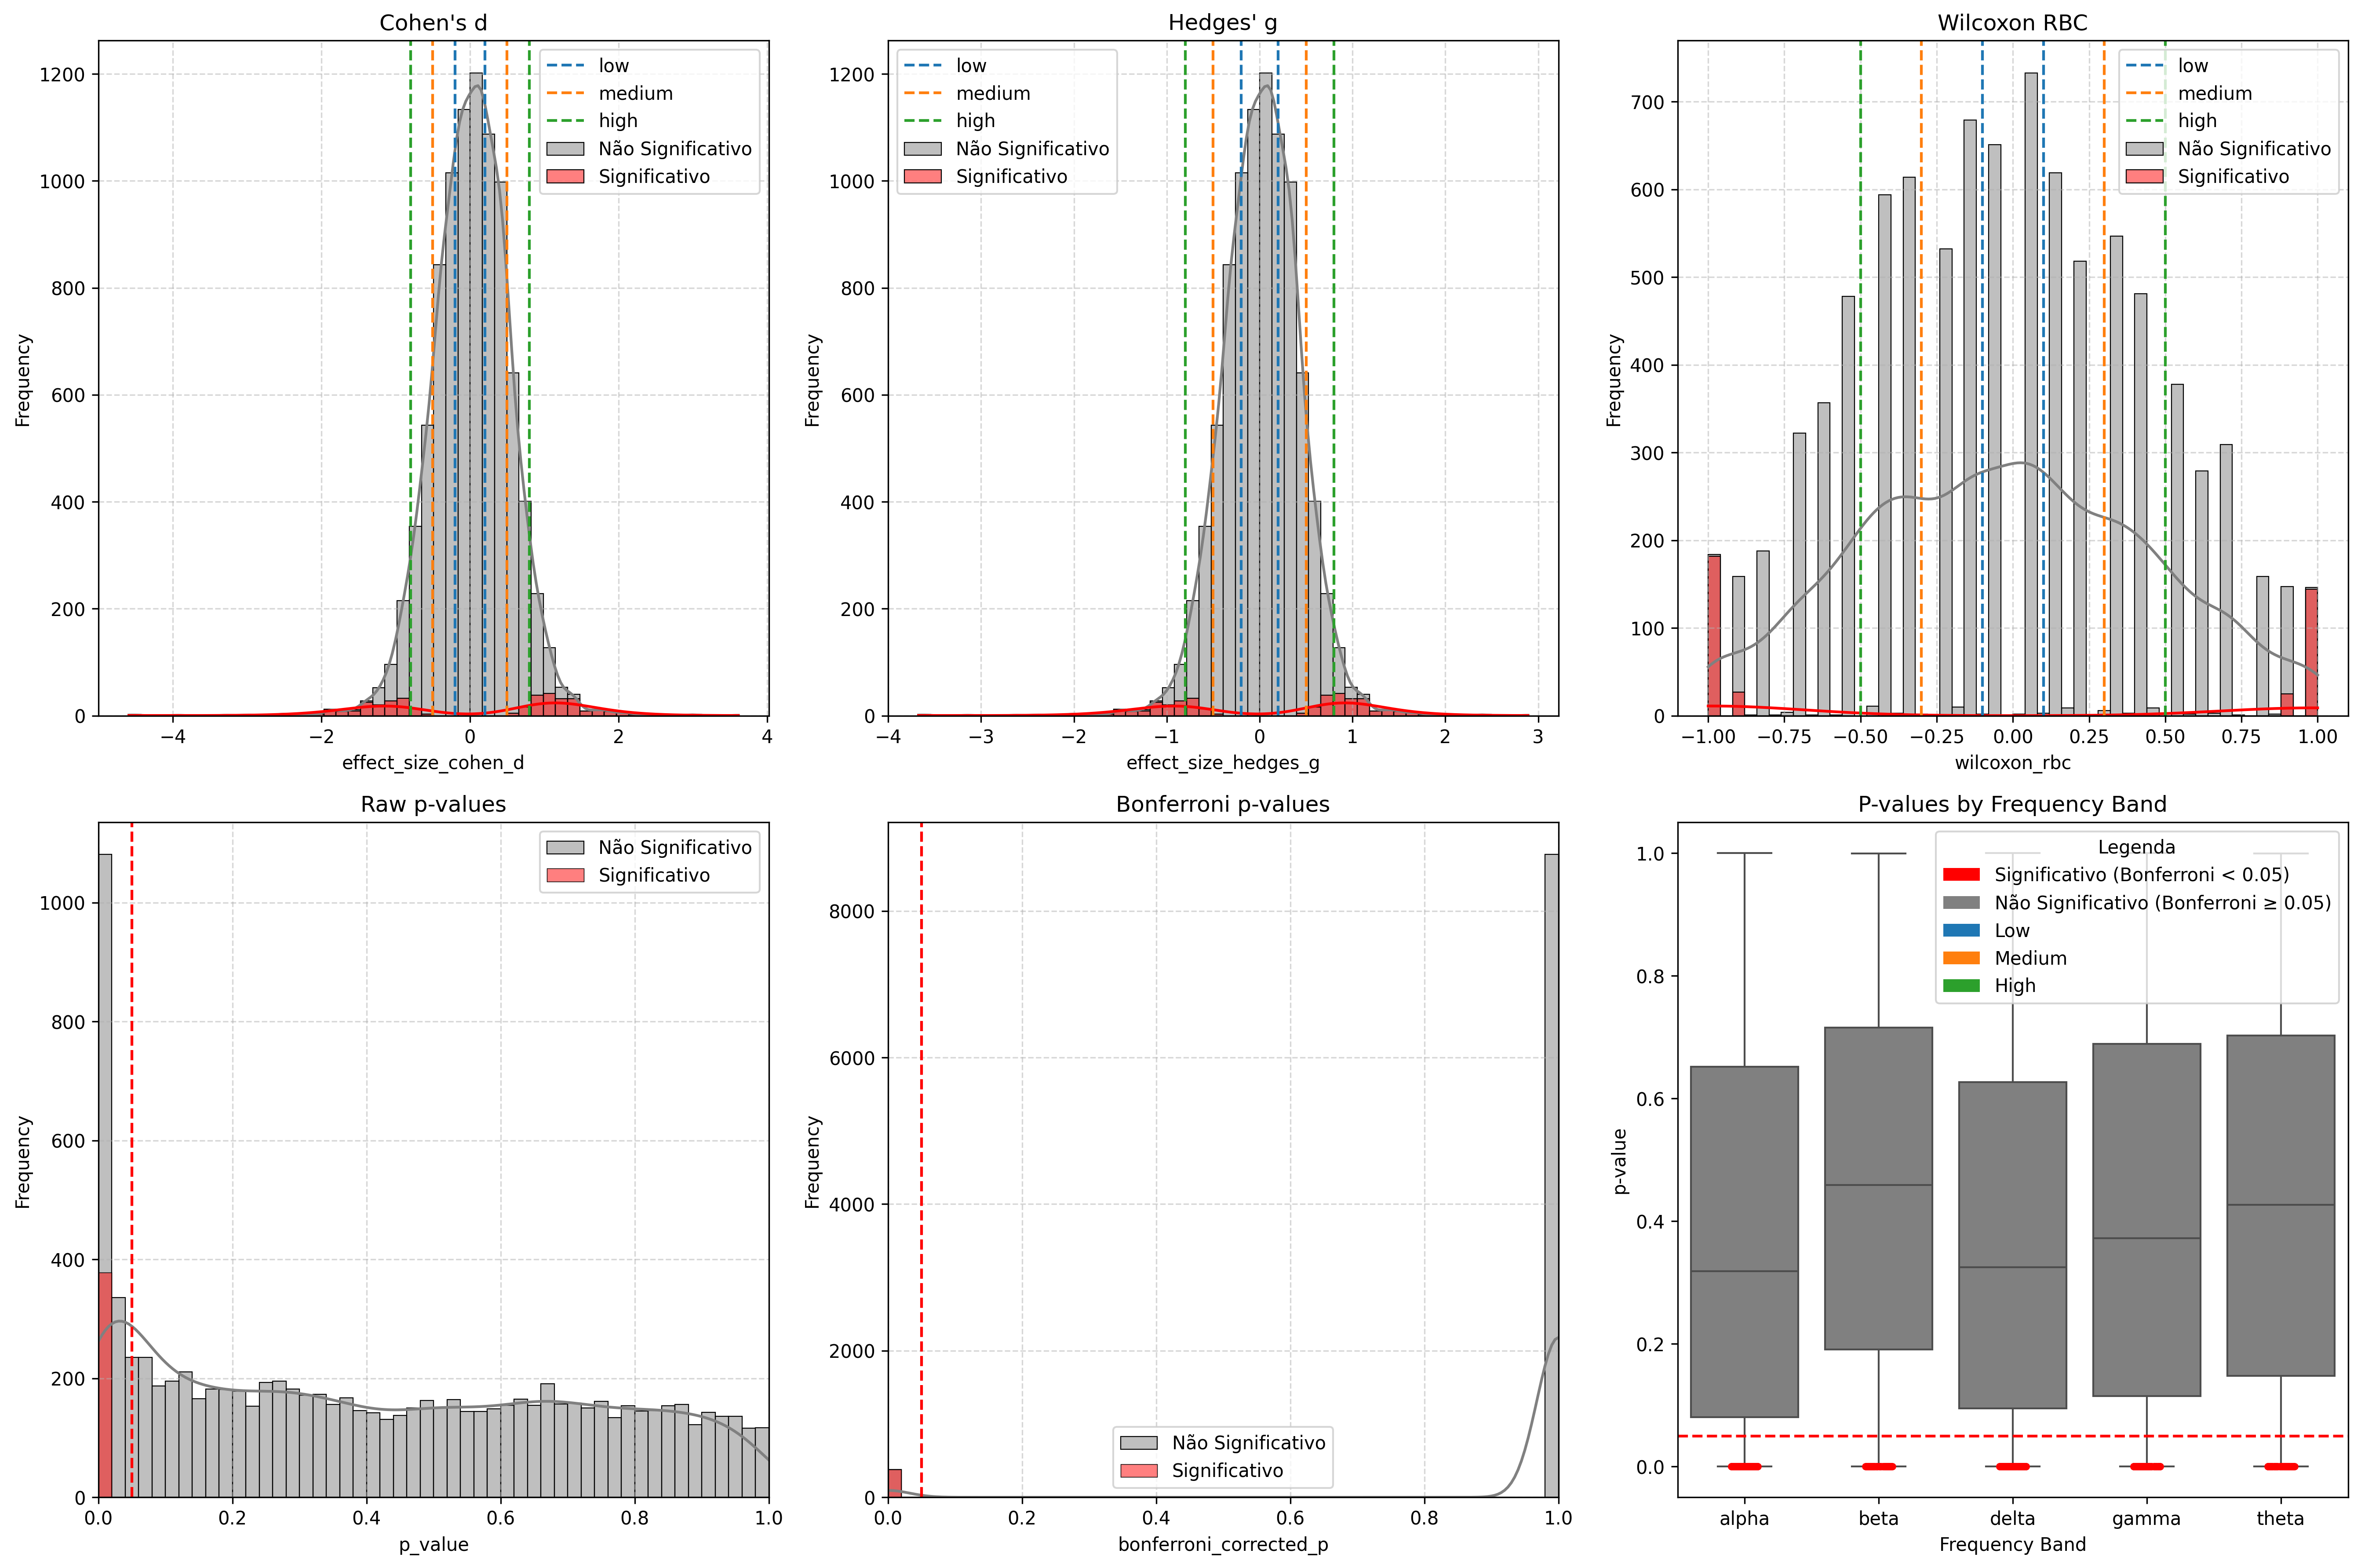
\includegraphics[width=0.45\textwidth]{figs/7_bootstrap_results_analysis/1_effect_size_histograms/Effect_Size_Histograms_PLI_EEGEEG_Com_Outliers.png}
    }
    \quad
    % Subfigura 4: CF-PLM (EEG-ECG), Com Outliers
    \subfloat[Com Outliers - CF-PLM (EEG-ECG)]{
        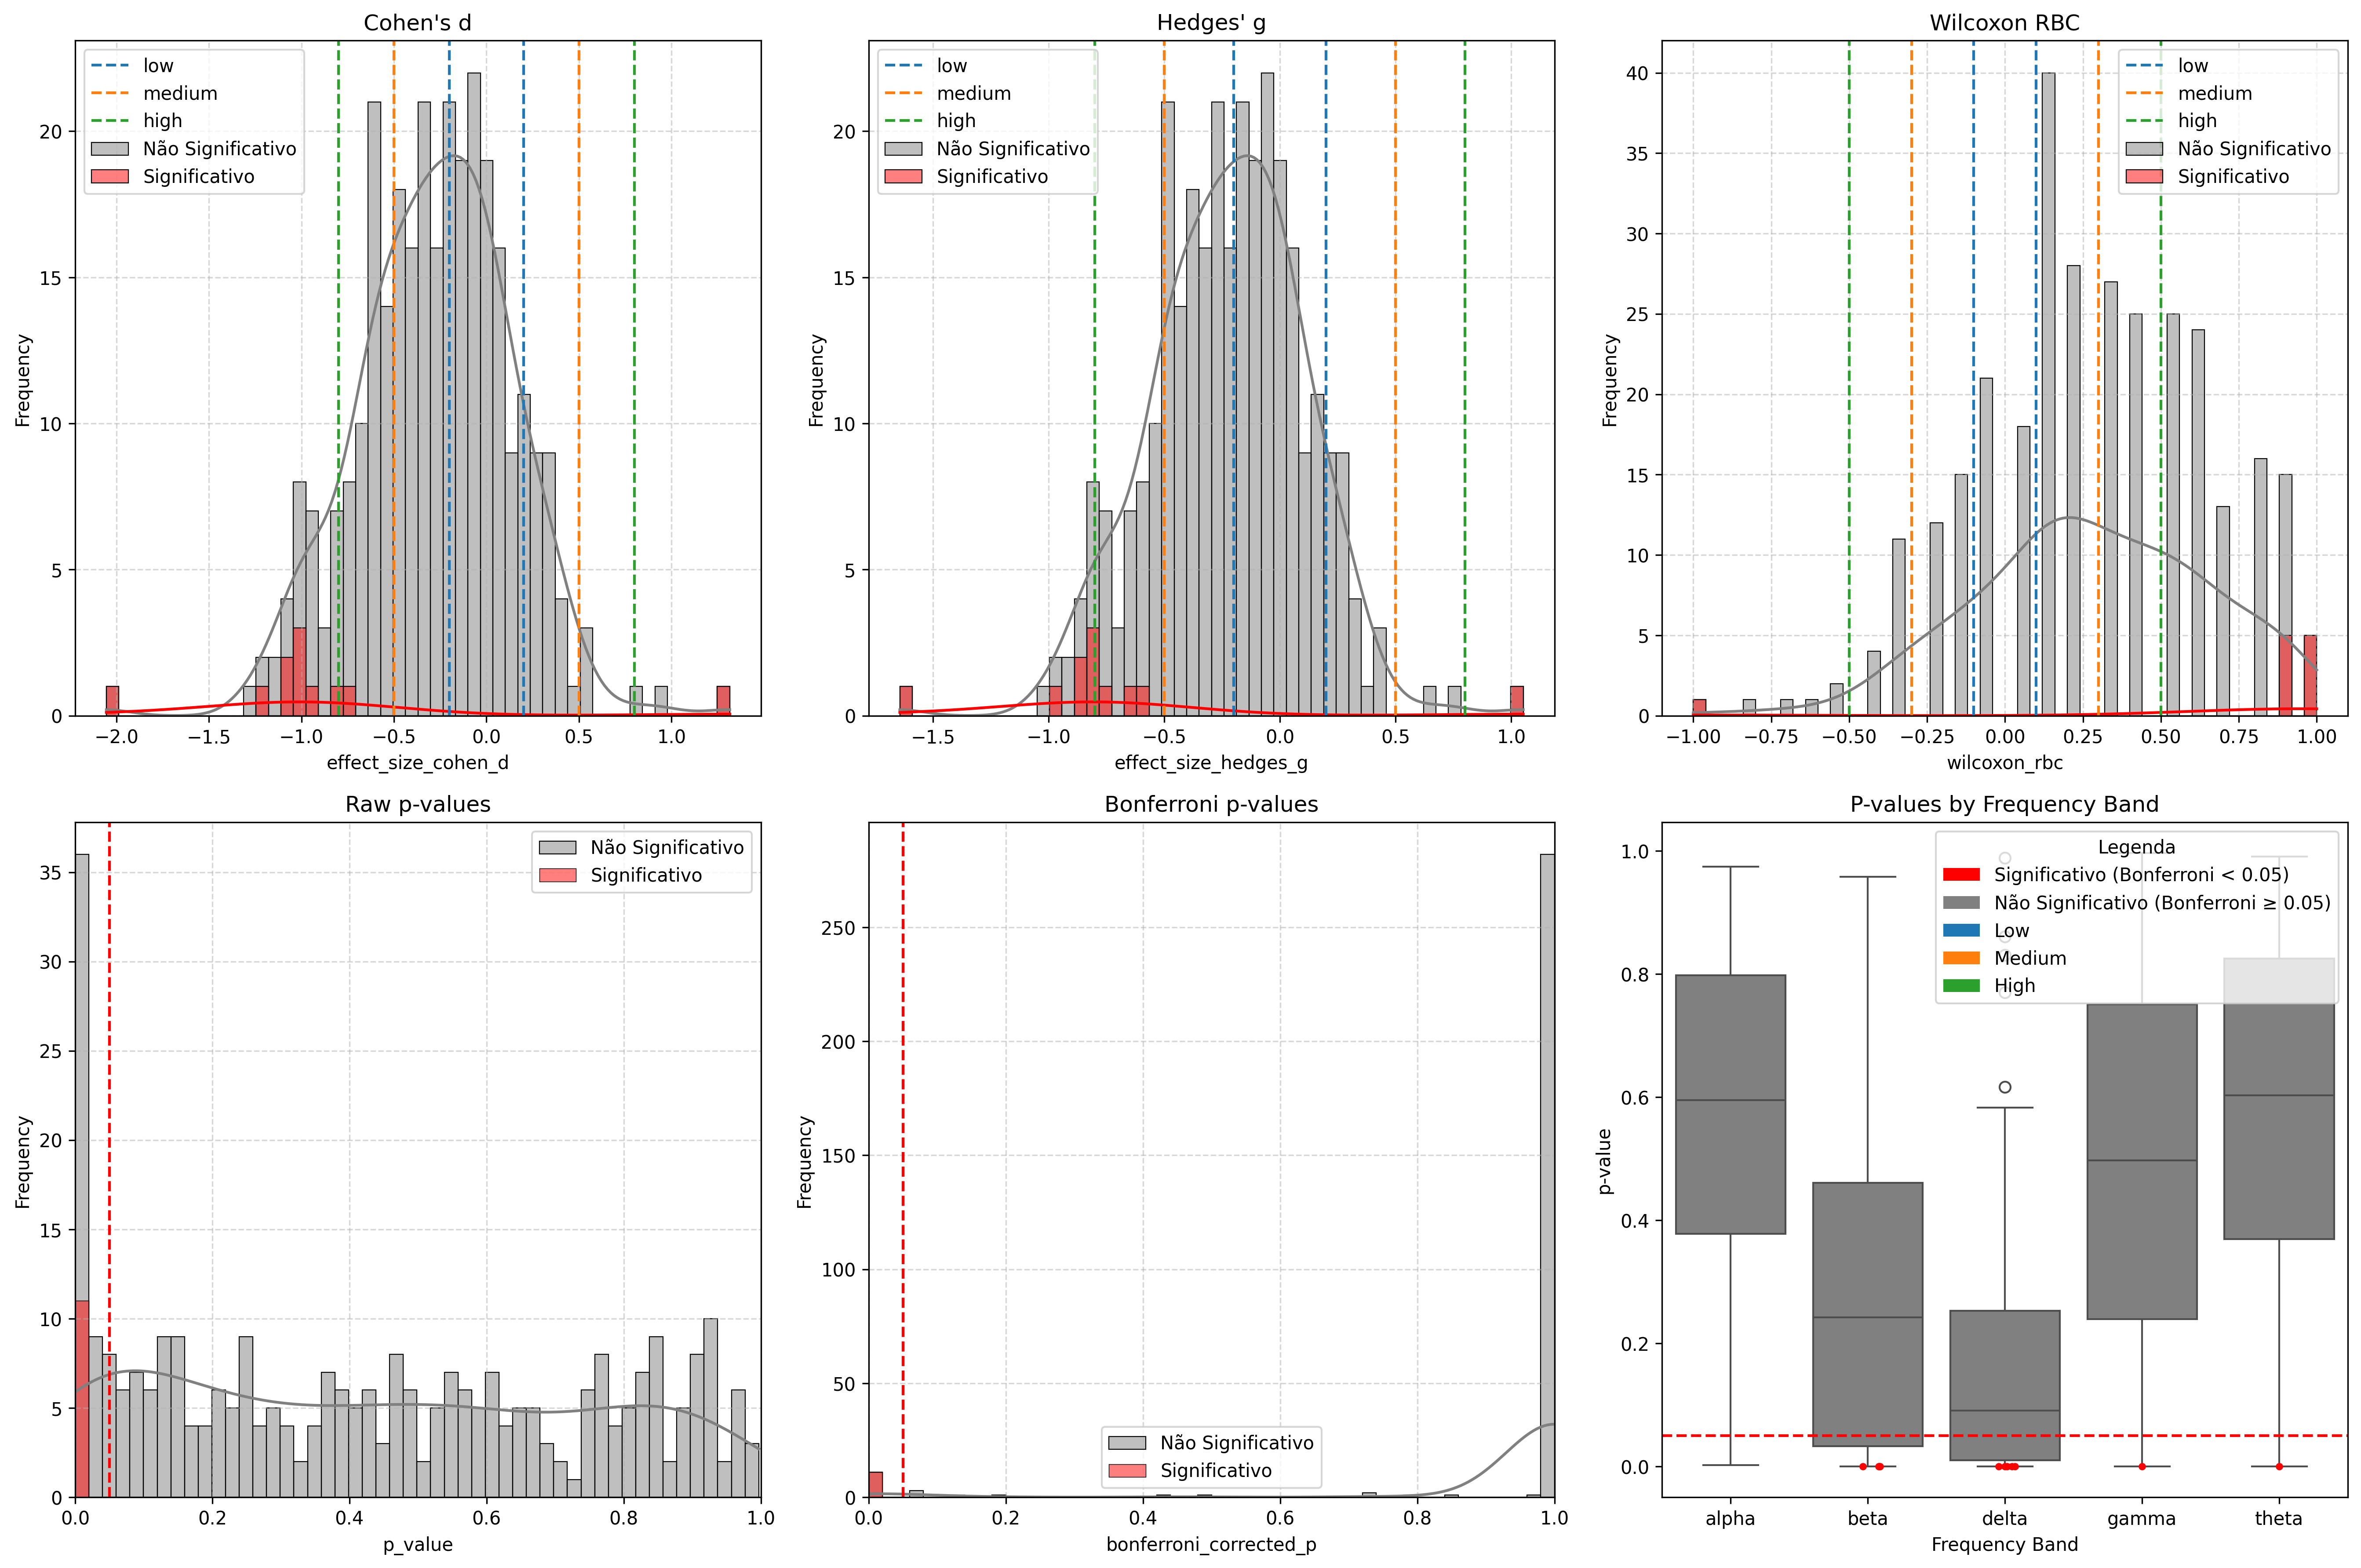
\includegraphics[width=0.45\textwidth]{figs/7_bootstrap_results_analysis/1_effect_size_histograms/Effect_Size_Histograms_CFPLM_EEGECG_Com_Outliers.png}
    }
    \caption[Distribuições de tamanhos de efeito e p-valores]{Distribuição das métricas de tamanho de efeito (Cohen's \(d\), Hedges' \(g\)  e Wilcoxon RBC) e dos p-valores (brutos e corrigidos por Bonferroni) para PLI (EEG-EEG) e CF-PLM (EEG-ECG), em cenários com e sem \textit{outliers}. O Wilcoxon RBC e o p-valor corrigido por Bonferroni (vertical tracejada vermelha em $p=0.05$) foram escolhidos como as métricas para representar, respectivamente, o tamanho do efeito e a significância estatística nas análises subsequentes.}
    \label{fig:effectsizehist_all}    
\end{figure}

\subsection{Distribuição dos Tamanhos de Efeito}
\subsubsection{Cohen's \(d\) e Hedges' \(g\) }
\begin{itemize}
    \item A maior parte dos valores concentra-se em torno de zero, indicando que, para a maioria dos pares, as diferenças entre as condições \textit{cathodic} e \textit{sham} são pequenas ou não significativas.
    \item Valores significativos (representados pelas barras vermelhas nos histogramas) tendem a se afastar de zero, sinalizando diferenças mais acentuadas. Por exemplo, valores de Cohen's \(d\) ou Hedges' \(g\)  superiores a 0.5 (ou inferiores a -0.5) sugerem um efeito moderado, enquanto valores acima de 0.8 (ou inferiores a -0.8) indicam um efeito alto.
    \item Embora Hedges' \(g\)  difira de Cohen's \(d\) ao aplicar uma correção para tamanhos amostrais pequenos, ambas as métricas exibem comportamentos semelhantes nos histogramas.
\end{itemize}

\subsubsection{\textit{Wilcoxon Rank-Biserial Correlation} (Wilcoxon RBC)}
\begin{itemize}
    \item O Wilcoxon RBC é derivado do teste não paramétrico de Wilcoxon e reflete a correlação de postos entre as condições, tipicamente variando de -1 a +1.
    \item Por não exigir pressupostos de normalidade, o RBC se mostra mais robusto no tratamento de dados heterogêneos e na presença de \textit{outliers}.
    \item Valores acima de 0.3 ou abaixo de -0.3 sugerem um efeito moderado; valores acima de 0.5 (ou abaixo de -0.5) indicam um efeito alto, e quando se aproximam de ±1, as condições diferem de forma quase absoluta.
    \item Devido a essa robustez, o RBC foi escolhido como nosso principal indicador de tamanho de efeito nas análises subsequentes.
\end{itemize}

\subsection{Distribuição de p-valores (Brutos e Corrigidos)}
\begin{itemize}
    \item Os histogramas de p-valores brutos mostram uma forte concentração em torno de 1 (indicando resultados não significativos) e uma cauda próxima de 0 (sinalizando potenciais resultados significativos).
    \item Após a correção de Bonferroni (indicada pela linha vertical tracejada em \(p=0.05\)), muitos dos valores que eram marginalmente significativos foram deslocados para a região de não significância, evidenciando o caráter conservador deste método de correção.
    \item Devido ao elevado número de comparações, a utilização do método Bonferroni minimiza a probabilidade de falsos positivos, sendo adotado como critério principal para a significância estatística.
\end{itemize}

\subsection{Comparação Entre Cenários (Com e Sem Outliers)}
\begin{itemize}
    \item \textbf{Impacto da Remoção de \textit{Outliers}:} De modo geral, a remoção de \textit{outliers} reduz ligeiramente o número de casos significativos em EEG-EEG, mas não altera substancialmente a distribuição dos tamanhos de efeito ou dos p-valores. No caso do EEG-ECG, a diferença entre manter ou remover \textit{outliers} é mínima, indicando que a presença de valores extremos tem pouco impacto na detecção de efeitos significativos nesse grupo.
    \item \textbf{PLI (EEG-EEG):} Cada par de canais EEG é único, totalizando \(\binom{61}{2}=1830\) pares por banda. Com 5 bandas e 6 atletas, temos \(1830\times6\times5=54900\) comparações.
    \item \textbf{CF-PLM (EEG-ECG):} Cada um dos 61 canais EEG é comparado ao canal ECG, totalizando \(61\) pares por banda. Com 5 bandas e 6 atletas, obtemos \(61\times6\times5=1830\) comparações.
    \item \textbf{Robustez do RBC e do Bonferroni:} Independentemente da remoção de \textit{outliers}, as comparações que apresentam valores elevados de Wilcoxon RBC e p-valores corrigidos abaixo de \( 0.05 \) permanecem confiáveis. Isso reforça a utilidade dessas métricas como principais indicadores da magnitude e significância estatística dos efeitos encontrados, independentemente da heterogeneidade dos dados.
\end{itemize}

Em resumo, os histogramas de Wilcoxon RBC (indicador de tamanho de efeito) e os p-valores corrigidos por Bonferroni (indicador de significância estatística) evidenciam quais pares de canais apresentam diferenças robustas entre as condições \textit{cathodic} e \textit{sham}. Embora Cohen's \(d\) e Hedges' \(g\)  também sejam úteis para quantificar a magnitude do efeito, enfatizamos o RBC devido à sua robustez, natureza não paramétrica e resiliência à heterogeneidade dos dados. Esses resultados fornecem uma base sólida para as análises topográficas e de rede apresentadas nas seções seguintes.

\subsection{Conclusões Principais}
\begin{itemize}
    \item A distribuição dos dados mostra que a maioria dos pares de canais apresenta diferenças pequenas entre as condições, com os valores de tamanho de efeito concentrando-se em torno de zero. Esse comportamento é esperado, dado o alto número de comparações e a aplicação de métodos rigorosos de correção múltipla, como Bonferroni.
    
    \item Nos casos onde há significância estatística, os tamanhos de efeito se afastam de zero de forma mais pronunciada (conforme evidenciado por Cohen's \(d\), Hedges' \(g\)  ou RBC), indicando diferenças que podem ser relevantes do ponto de vista da dinâmica de conectividade funcional.

    \item O Wilcoxon RBC se destaca como a métrica escolhida para quantificar tanto a direção quanto a magnitude das diferenças, sem assumir pressupostos de normalidade. Essa característica torna o RBC uma escolha apropriada para as próximas etapas da análise, que incluem a caracterização topográfica e a construção dos grafos de conectividade.

\end{itemize}

Dessa forma, a análise dos histogramas de tamanhos de efeito e dos p-valores fornece um panorama inicial detalhado. Embora a maioria dos pares de canais não apresente diferenças significativas, observa-se um conjunto de casos com efeitos inicialmente moderados ou altos, mas que, após a correção para múltiplas comparações, se restringem predominantemente aos valores de efeito mais elevados. Esses achados servem como base para investigações posteriores, focadas na identificação de padrões espaciais e espectrais na neuromodulação, contribuindo para uma compreensão mais aprofundada das interações entre EEG e ECG nas condições experimentais avaliadas.